\documentclass[legalpaper, 11pt,spanish]{article}
\usepackage[utf8]{inputenc}
\usepackage{babel}
\usepackage{fullpage}
\usepackage{listings}
\usepackage{mathpazo}
\usepackage{enumitem}
\usepackage{courier}
\usepackage{xcolor}
\usepackage{textcomp}
\usepackage{amsmath}
\usepackage{amssymb}
\usepackage{tikz}
\usepackage{fancyhdr}
\usepackage{graphics}
\usepackage{wrapfig}
\usetikzlibrary{calc,patterns,arrows}

\hyphenation{arre-glos dife-rencias tempe-ra-turas}

\newcommand{\titulo}{Certamen 3, sábado 18 de junio de 2011}
\newcommand{\cc}[1]{\hfil\texttt{#1}\hfil}
\newcommand{\pond}[1]{[{\small\textbf{#1\%}}]}

\pagestyle{fancy}
\lhead{%
  {\Large\bfseries Programación---\titulo} \\
  Nombre: \nombre\hfill
  Rol:    \rol
  \vspace{2ex}
}
\chead{}\rhead{}\lfoot{}\cfoot{}\rfoot{}
\renewcommand{\headrulewidth}{0pt}
\addtolength{\headheight}{7ex}
\headsep=4ex


\newcommand{\onelinerule}{\rule[2.3ex]{0pt}{0pt}}
\newcommand{\twolinerule}{\rule[6.2ex]{0pt}{0pt}}
\newcommand{\respuesta}{\framebox[\textwidth]{\twolinerule}}
\newcommand{\nombre}{%
  \begin{tikzpicture}[xscale=.4,yscale=.7]
    \draw (0, 0) rectangle (22, 1);
  \end{tikzpicture}%
}
%\newcommand{\rol}   {\framebox[0.3\textwidth]{\onelinerule}}
\newcommand{\rol}{%
  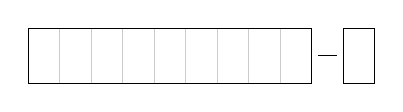
\begin{tikzpicture}[xscale=.4,yscale=.7]
    \draw[gray!40] ( 0, 0) grid      ( 9, 1);
    \draw          ( 0, 0) rectangle ( 9, 1);
    \draw          (10, 0) rectangle (11, 1);
    \draw (9 + .2, .5) -- (10 - .2, .5);
  \end{tikzpicture}%
}
\newcommand{\li}{\lstinline}
\providecommand{\pond}[1]{[{\small\textbf{#1\%}}]}

\lstdefinelanguage{py}{%
  classoffset=0,%
    morekeywords={%
      False,class,finally,is,return,None,continue,for,lambda,try,%
      True,def,from,nonlocal,while,and,del,global,not,with,print,%
      as,elif,if,or,yield,assert,else,import,pass,break,except,in,raise},%
    keywordstyle=\color{black!80}\bfseries,%
  classoffset=1,
    morekeywords={int,float,str,abs,len,raw_input,exit,range,min,max,%
      set,dict,tuple,list,bool,complex,round,sum,all,any,zip,map,filter,%
      sorted,reversed,dir,file,frozenset,open,%
      array,zeros,ones,arange,linspace,eye,diag,dot},
    keywordstyle=\color{black!50}\bfseries,%
  classoffset=0,%
  sensitive=true,%
  morecomment=[l]\#,%
  morestring=[b]',%
  morestring=[b]",%
  stringstyle=\em,%
}

\lstdefinelanguage{testcase}{%
  moredelim=[is][\bfseries]{`}{`},%
  backgroundcolor=\color{gray!20},%
}

\lstdefinelanguage{file}{%
  frame=single,%
}

\lstset{language=py}
\lstset{basicstyle=\ttfamily}
\lstset{columns=fixed}
\lstset{upquote=true}
\lstset{showstringspaces=false}
\lstset{rangeprefix=\#\ }
\lstset{includerangemarker=false}

\newlist{certamen}{enumerate}{1}
\setlist[certamen]{%
  label=\arabic*.,
  font=\LARGE\bfseries,%
  labelindent=-.5in,%
  leftmargin=0pt,%
  labelsep=1em%
}



\begin{document}

  \begin{enumerate}[font=\Large\bfseries]

    \item
      \pond{25}
      Indique qué es lo que imprimen los siguientes programas.

      \foreach \x in {1,2,...,6} {
        \noindent
        \begin{minipage}[b]{19.8em}
          \lstinputlisting[linerange=INICIO-]{p\x.py}
          \framebox[18em]{\rule[9ex]{0pt}{0pt}}
          \vspace{0.7em}
        \end{minipage}
      }

      Dibuje la ventana que resulta al ejecutar
      el siguiente programa.

      %\foreach \x in {7,8} {
      %  \noindent
      %  \begin{minipage}[b]{19.8em}
      %    \lstinputlisting{p\x.py}
      %    \framebox[18em]{\rule[6ex]{0pt}{0pt}}
      %    \vspace{0.7em}
      %  \end{minipage}
      %}

      \begin{minipage}[b]{19.8em}
        \lstinputlisting{p8.py}
      \end{minipage}
      \hfil
      \begin{minipage}[b]{16em}
        \framebox[\textwidth]{\rule[30ex]{0pt}{0pt}}
      \end{minipage}

    \newpage
    \item
      \pond{25}
      Una \emph{serie de tiempo}
      es una secuencia de valores numéricos
      obtenidos al medir algún fenómeno cada cierto tiempo.
      Algunos ejemplos de series de tiempo son:
      el precio del dólar en cada segundo,
      el nivel medio mensual de concentración de CO\(_2\) en el aire y
      las temperaturas máximas anuales de una ciudad.
      En un programa, los valores de una serie de tiempo se pueden guardar en un arreglo.

      \begin{enumerate}
        \item Las \emph{medias móviles con retardo \(p\)} de una serie de tiempo
          son la secuencia de todos los promedios de \(p\)~valores consecutivos de la serie.

          %Por ejemplo,
          %si los valores de la serie son \(\{5, 2, 2, 8, -4, -1, 2\}\),
          %entonces las medias móviles con retardo 3 son
          %\(\frac{5 + 2 + 2}{3}\),
          %\(\frac{2 + 2 + 8}{3}\),
          %\(\frac{2 + 8 - 4}{3}\),
          %\(\frac{8 - 4 - 1}{3}\) y
          %\(\frac{-4 -1 + 2}{3}\).

          Escriba la función \li!medias_moviles(serie, p)!
          que retorne el arreglo de las medias móviles con retardo~\(p\) de la serie:
          \begin{lstlisting}
>>> s = array([5, 2, 2, 8, -4, -1, 2])
>>> medias_moviles(s, 3)
array([ 3,  4,  2,  1, -1])
          \end{lstlisting}

          En este ejemplo,
          las medias móviles son:
          \(\frac{5 + 2 + 2}{3}\),
          \(\frac{2 + 2 + 8}{3}\),
          \(\frac{2 + 8 - 4}{3}\),
          etc.

        \item Las \emph{diferencias finitas} de una serie de tiempo
          son la secuencia de todas las diferencias entre un valor y el anterior.

          %Por ejemplo,
          %si los valores de la serie son \(\{5, 2, 2, 8, -4, -1, 2\}\),
          %entonces las diferencias finitas son:
          %\((2 - 5)\),
          %\((2 - 2)\),
          %\((8 - 2)\),
          %\((-4 - 8)\),
          %\((-1 + 4)\) y
          %\((2 + 1)\).

          Escriba la función \li!diferencias_finitas(serie)!
          que retorne el arreglo de las diferencias finitas de la serie:
          \begin{lstlisting}
>>> s = array([5, 2, 2, 8, -4, -1, 2])
>>> diferencias_finitas(s)
array([ -3,   0,   6, -12,   3,   3])
          \end{lstlisting}

        %\item El \emph{suavizado exponencial con factor \(\alpha\)} de una serie de tiempo
        %  es una nueva serie de tiempo
      \end{enumerate}

    \newpage
    \item
      \pond{25}
      Alicia y Benito usan un programa para llevar la cuenta
      del marcador de sus partidos de tenis de mesa.
      Cada vez que alguno de ellos gana un punto,
      hace clic en el botón con su nombre,
      y el marcador es actualizado.

      Un partido de tenis de mesa está dividido en 7 juegos.
      Cuando alguien gana 11 puntos,
      el juego se termina y comienza el juego siguiente.

      \begin{tikzpicture}[scale=5.5]
        \node (A) at (0, 0) {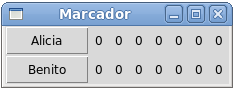
\includegraphics[scale=0.55]{marcador-0.png}};
        \node (B) at (1, 0) {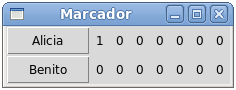
\includegraphics[scale=0.55]{marcador-1.png}};
        \node (C) at (2, 0) {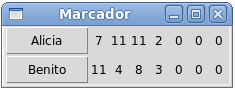
\includegraphics[scale=0.55]{marcador-2.png}};
        \draw[-latex'] (A) -- (B);
        \draw[-latex'] (B) -- (C);
        \node[font=\footnotesize, anchor=baseline, node distance=6ex, below of=A] {Marcador inicial};
        \node[font=\footnotesize, anchor=baseline, node distance=6ex, below of=B] {Después de hacer clic en Alicia};
        \node[font=\footnotesize, anchor=baseline, node distance=6ex, below of=C] {Después de muchos clics};
      \end{tikzpicture}

      El programa define dos listas de modelos,
      llamadas \li!modelos_a! y \li!modelos_b!,
      que guardan los puntos ganados en cada juego
      por el jugador respectivo.
      Por ejemplo, \li!modelos_a[3]! guarda los puntos
      que ha ganado Alicia en el cuarto juego
      (recuerde que se cuenta desde cero).

      Además,
      hay un modelo que guarda cuál es el juego actual
      (un número entre 0 y 6):
      \lstinputlisting[linerange=JUEGO\ ACTUAL-FIN\ JUEGO\ ACTUAL]{pauta-marcador.py}

      Los botones fueron creados de la siguiente manera:
      \lstinputlisting[linerange=BOTONES-FIN\ BOTONES]{pauta-marcador.py}

      Escriba el código del controlador \li!punto_a!.

    \newpage
    \item
      \pond{25}
      Las imágenes en tonos de grises (por ejemplo, una foto en blanco y negro)
      son matrices de valores entre 0 y 255.
      Cada elemento de la matriz se denomina \emph{píxel}.
      El valor 0 representa el negro, el 255 el blanco, y los valores intermedios
      las distintas intensidades de grises.

      \begin{center}
        \begin{tikzpicture}[yscale=-1, scale=.10]
          \begin{scope}
            \node[anchor=north west, inner sep=0pt] at (0, 0) {
\includegraphics[scale=5.9]{utfsm.png}};
            \draw[very thin] (0, 0) grid (45, 27);
            \draw[step=3cm] (0, 0) grid (45, 27);
            \node[ultra thick, draw=red!80!black, inner sep=5pt] (A) at (34.5, 19.5) {};
            \node[anchor=north] at ({45 / 2}, 27) {\texttt{img}};
          \end{scope}
          \begin{scope}[xshift=65cm, yshift=18cm]
            \node[anchor=north west, inner sep=0pt] at (0, 0) {
\includegraphics[scale=5.87]{utfsm-chica.png}};
            \draw[very thin] (0, 0) grid (15, 9);
            \node[very thick, draw=red!80!black, inner sep=2pt] (B) at (11.5, 6.5) {};
            \node[anchor=north] at ({15 / 2}, 9) {\texttt{reducir(img, 3)}};
          \end{scope}
          \begin{scope}[xshift=100cm]
            \node[anchor=north west, inner sep=0pt] at (0, 0) {
\includegraphics[scale=5.89]{utfsm-bin.png}};
            \draw[very thin] (0, 0) grid (45, 27);
            \node[anchor=north] at ({45 / 2}, 27) {\texttt{binarizar(img, 146)}};
          \end{scope}
          \draw[very thick, -latex'] (A) to (B);
          %\draw[very thick, -latex', out=180] (A.north east) to (B.north west);
          %\draw[very thick, out=-45, in=-145, -latex'] (A.north east) to (B.north west);
        \end{tikzpicture}
      \end{center}

      \begin{enumerate}
        \item
          Un método para reducir \(f\) veces el tamaño de una imagen
          es partir la imagen en bloques de \(f\times f\)
          y promediar los valores de los píxeles de cada bloque.
          Este promedio será el valor del píxel correspondiente en la nueva imagen.
          Si la imagen original es de \(m\times n\) píxeles,
          la imagen reducida quedará de \((m/f) \times (n/f)\) píxeles.

          Escriba la función \li!reducir(img, f)!,
          donde \li!img! es una imagen (es decir, una matriz),
          que retorne una nueva imagen
          que sea \li!img! reducida en un factor de \li!f!.

        \item
          La \emph{binarización} de una imagen
          consiste en crear una nueva imagen cuyos píxeles sólo son negros o blancos.
          Para esto se escoge un valor llamado \emph{umbral};
          todos los píxeles mayores o iguales que el umbral quedan blancos,
          y los menores al umbral quedan negros.

          Escriba la función \li!binarizar(img, umbral)!
          que retorne una nueva imagen
          que sea una versión binarizada de \li!img! de acuerdo al umbral indicado.
      \end{enumerate}

  \end{enumerate}
\end{document}

